\documentclass[10pt]{beamer}

% Paquetes
\usepackage[T1]{fontenc}    % Para escribir en español
\usepackage[spanish]{babel}
\usepackage{hyperref}    % Para hacer links a la web
\usepackage{listings}    % Para incluir código

% Setup imagenes
\graphicspath{ {out/}}

\setlength{\abovecaptionskip}{-1pt plus 0pt minus 0pt}

% Estilos
\usetheme{Madrid}


% Personalización del footer
\setbeamertemplate{footline}{%
  \leavevmode%

  \hbox{\begin{beamercolorbox}[wd=.5\paperwidth, center, ht=2.25ex]{author in head/foot}%
    \usebeamerfont{author in head/foot}\insertshortauthor%
  \end{beamercolorbox}%

  \begin{beamercolorbox}[wd=.4\paperwidth, center, ht=2.25ex]{title in head/foot}%
    \usebeamerfont{title in head/foot}\insertshorttitle%
  \end{beamercolorbox}%

  \begin{beamercolorbox}[wd=.1\paperwidth, center, ht=2.25ex]{date in head/foot}%
    \insertframenumber{} / 15%%
  \end{beamercolorbox}
  }%

  \vskip0pt%
}%

% Eliminar barra de navegación
\beamertemplatenavigationsymbolsempty

% CAptions
\usepackage[font=footnotesize,labelfont=bf]{caption}
\setbeamertemplate{caption}[numbered]

% Info para la title page
\title{Concurrencia a Museos de Argentina}
\subtitle{Relación con otros consumos culturales}
\author{Nazareno Magallanes \and Javier Spina \and Lautaro Terreno}
\institute[ECyT]
{
  {\large Introducción a la Ciencia de Datos}
  \and
  Escuela de Ciencia y Tecnología
  \and
  Universidad Nacional de San Martín
}
\date{14 Noviembre 2022}


% Inicio del documento
\begin{document}

\frame{\titlepage}

% Pregunta y contexto
\begin{frame}
\frametitle{La pregunta y su contexto}

\begin{block}{La pregunta}
¿Cómo aumentar la concurrencia a los museos?
\end{block}

\begin{figure}
\centering
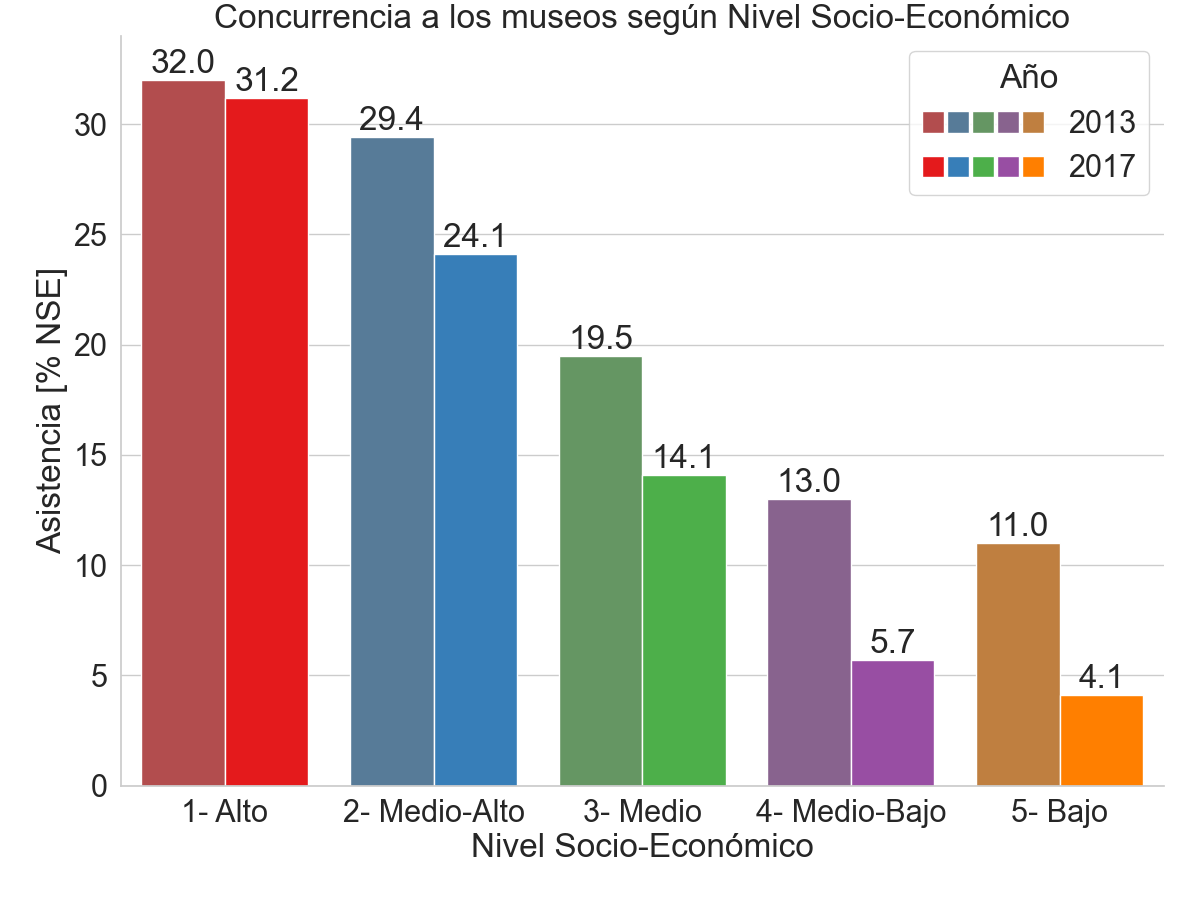
\includegraphics[height=0.6\textheight]{asist_museo_nse_x100}
\label{fig:asist_museo_nse}
\caption{Asistencia a museos 2013-2017}
\end{figure}

\end{frame}

% Presentación
\begin{frame}
\frametitle{Presentación del \textit{dataset}}

\begin{columns}
\column{0.5\textwidth}
\begin{figure}
\centering

\includegraphics[height=0.7\textheight]{encc_informe_portada.pdf}
\label{fig:portada_encc}
\end{figure}

\column{0.5\textwidth}
\begin{itemize}
\item Se trabajó con el \textit{dataset} asociado a la \textbf{Encuesta Nacional de Consumos Culturales} realizada en 2017. 
\item Se complementó con datos abiertos de los Museos de Argentina y un Shapefile de Argentina de las 23 provincias y CABA.
\end{itemize}
\end{columns}

\end{frame}

\begin{frame}
  \frametitle{Trabajo inicial: unidades y variables}
  \begin{columns}
    \column{0.2\textwidth}
      Encuesta\\
      2802 unidades\\
      450 variables
    \column{0.5\textwidth}
      \begin{figure}
        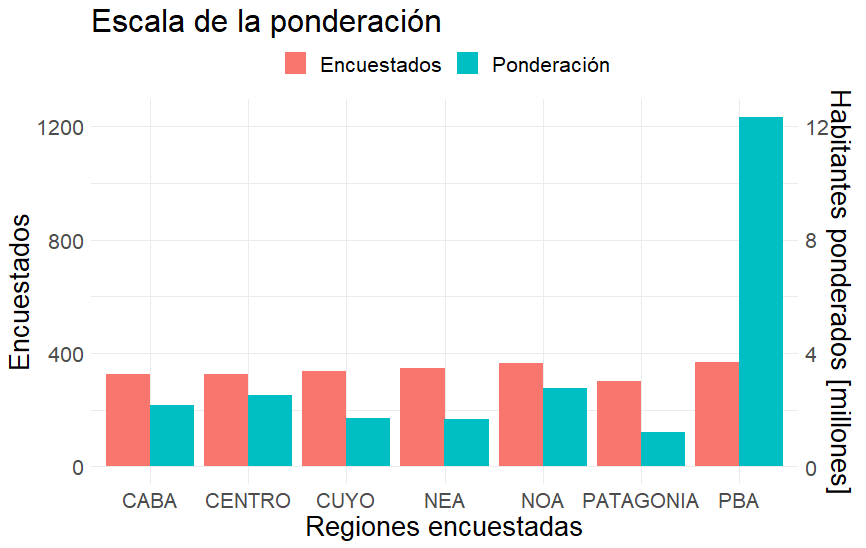
\includegraphics[width=\textwidth]{pondera}
        \label{fig:pondera}
        \caption{Importancia de la ponderación}
      \end{figure}
    \column{0.3\textwidth}
      \begin{figure}
        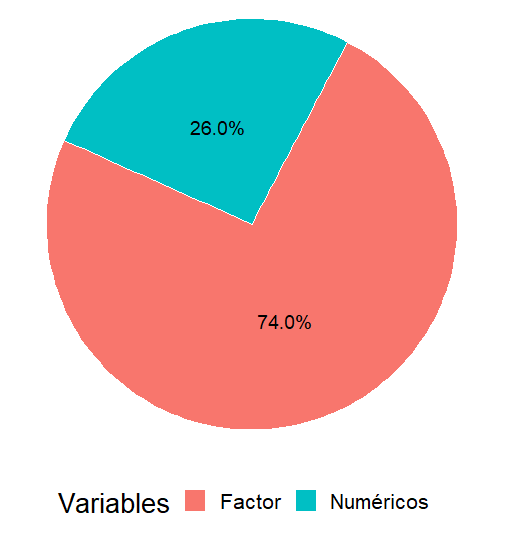
\includegraphics[width=0.8\textwidth]{tipos_variables}
        \label{fig:tipos_variables}
        \caption{Tipos de variables}
      \end{figure}
  \end{columns}

  \vfill

  \begin{columns}
    % \column{0.5\textwidth}
    % \begin{figure}
    %   \vspace{-2em}
    % 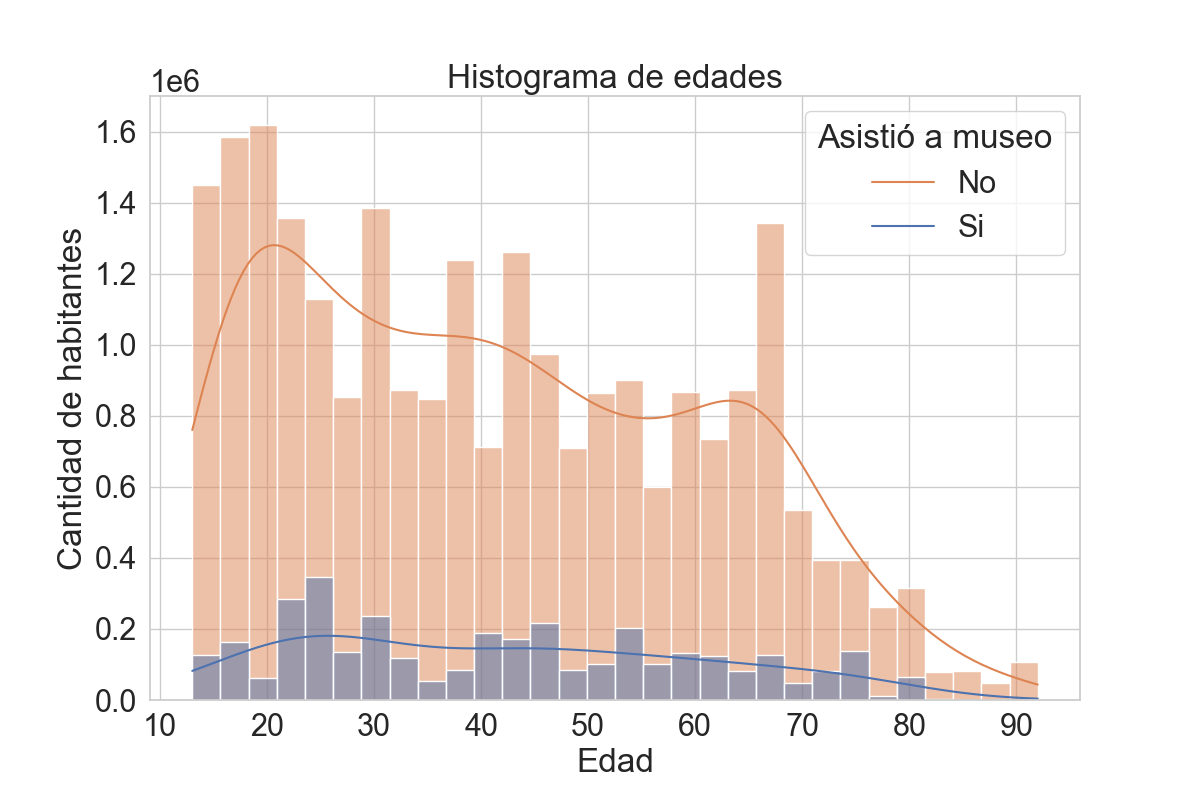
\includegraphics[width=0.9\textwidth]{histo_edades_concurrencia.png}
    % \label{fig:histo_edades}
    % \end{figure}
    \column{0.2\textwidth}
    Museos\\
    1182 unidades\\
    27 variables

    \column{0.3\textwidth}
    \resizebox{\textwidth}{!}{%
      \begin{tabular}{ |l|c| }
        \hline
        Localizacion & Unidades\\ \hline
        Precisa & 1179 \\ \hline
        Centroide de la localidad & 1 \\ \hline
        Centroide por proximidad & 2\\ \hline
      \end{tabular}}
      \column{0.45\textwidth}
      \begin{itemize}
        \item Se agregó la columna región en el \emph{dataset} de la ubicación de los museos.
        \item Se limitó el Shapefile de Argentina a la vista continental.
      \end{itemize}
  \end{columns}

\end{frame}

\begin{frame}
\frametitle{Análisis Exploratorio}

\begin{columns}
\column{0.5\textwidth}
\begin{figure}
\vspace{-2.75em}
\includegraphics[width=\textwidth]{museos_datosabiertos.png}
\label{fig:museos}
\caption{Argentina y sus museos}
\end{figure}
\column{0.5\textwidth}
\begin{figure}

  \vspace{-1.5em}
  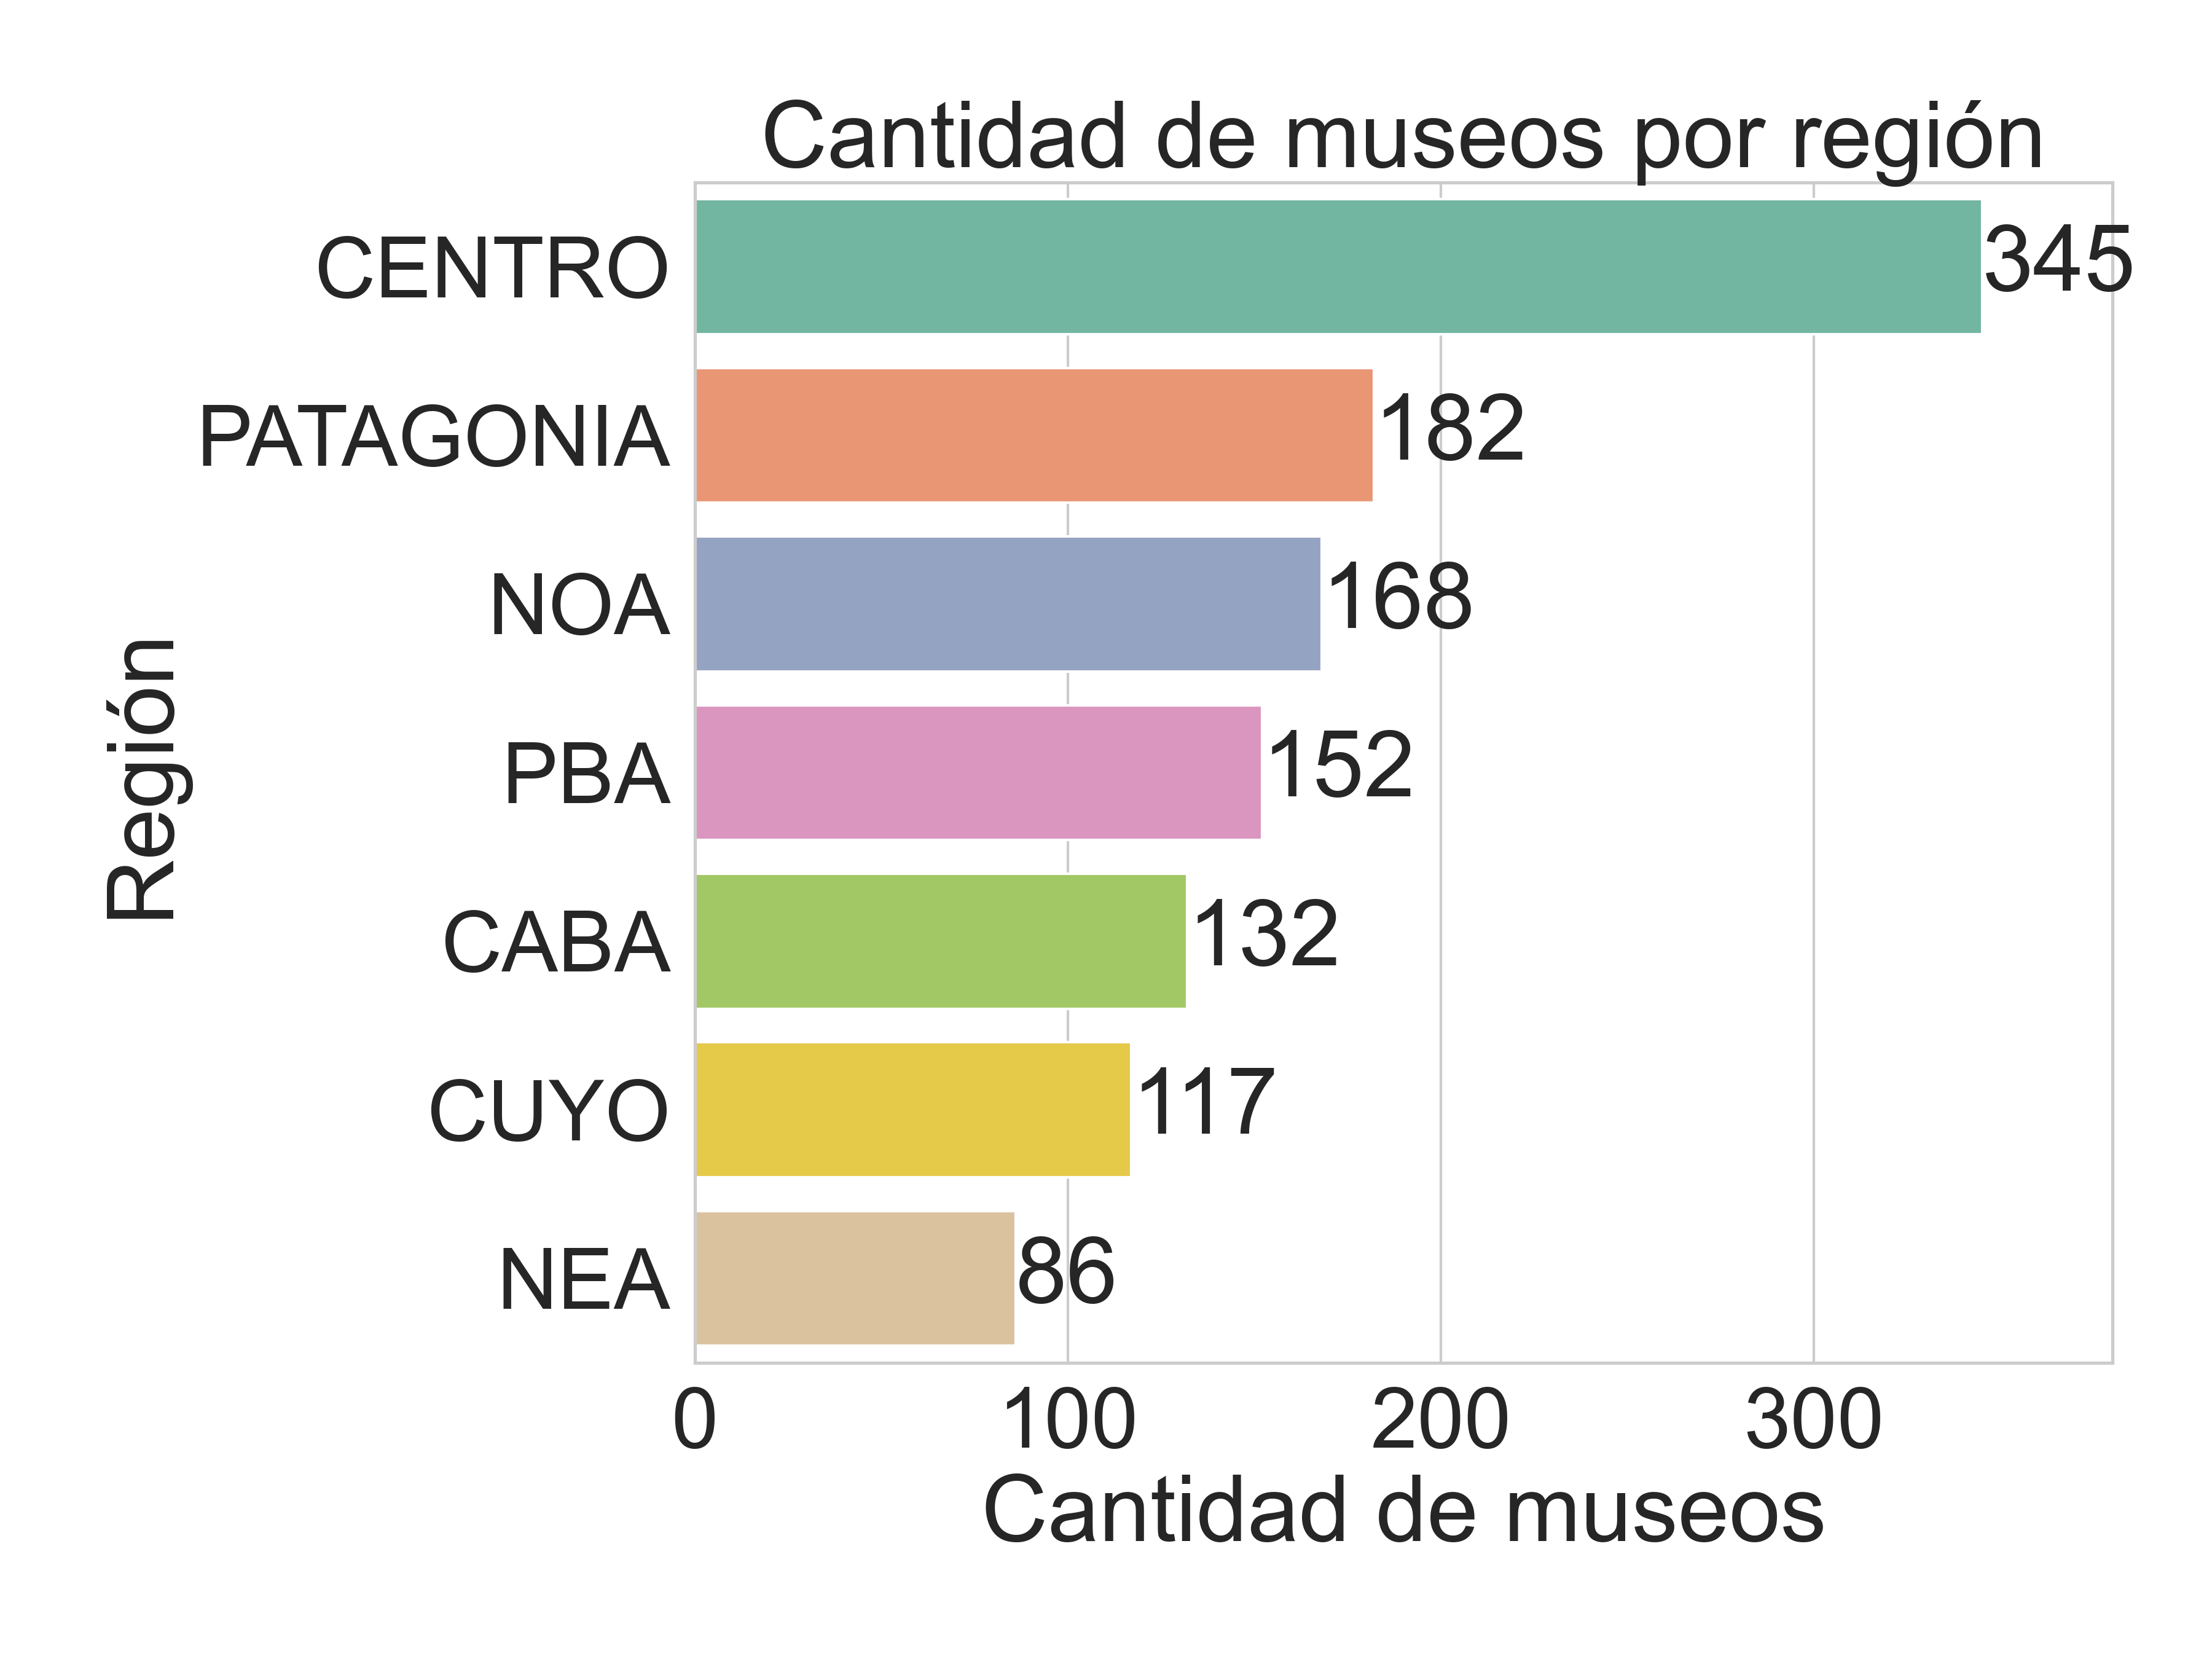
\includegraphics[width=0.9\textwidth]{cantidad_museos.png}
  \label{fig:cant_museos}
  \caption{Cantidad de museos por región}
\end{figure}
  \begin{figure}
    \vspace{-2.25em}
    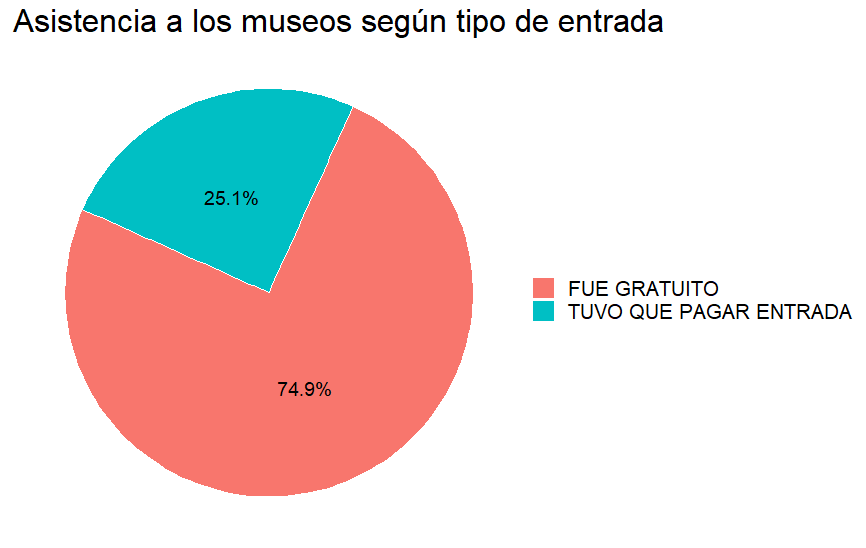
\includegraphics[width=0.9\textwidth]{entradas.png}
    \label{fig:tipos_entradas}
    \caption{Influencia de la gratuidad de la entrada}
    \end{figure}
\end{columns}

\end{frame}

\begin{frame}
  \frametitle{Análisis Exploratorio}
  \begin{figure}
    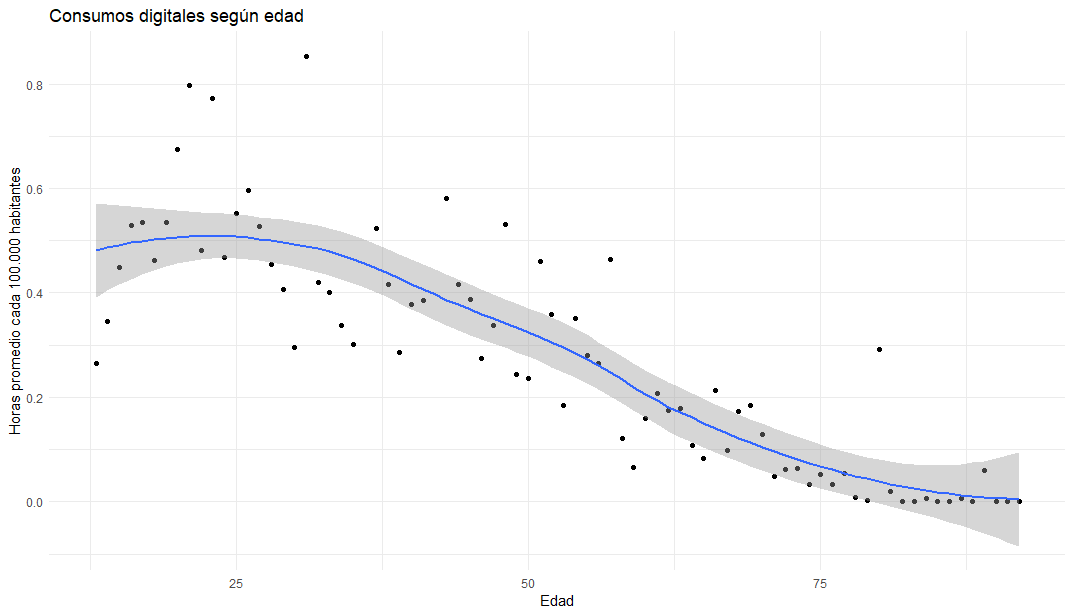
\includegraphics[width=\textwidth]{consumos_digitales.png}
    \label{fig:digitales}
    \caption{Consumos digitales según edad}
    \end{figure}
\end{frame}

\begin{frame}
  \frametitle{Análisis Específico}
  \begin{figure}
    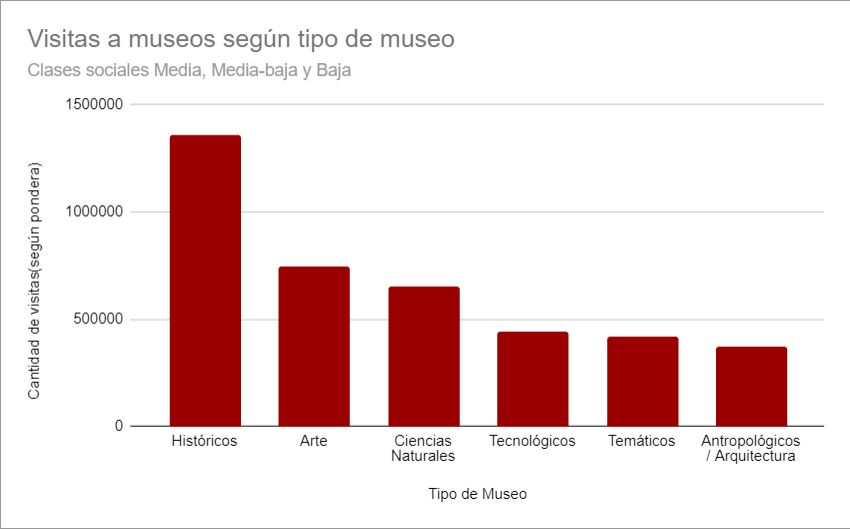
\includegraphics[width=0.95\textwidth]{visitas.jpg}
    \label{fig:visitas}
    \caption{Visitas a museos}
    \end{figure}
  \end{frame}

  \begin{frame}
    \frametitle{Análisis Específico}

  
    \begin{figure}
      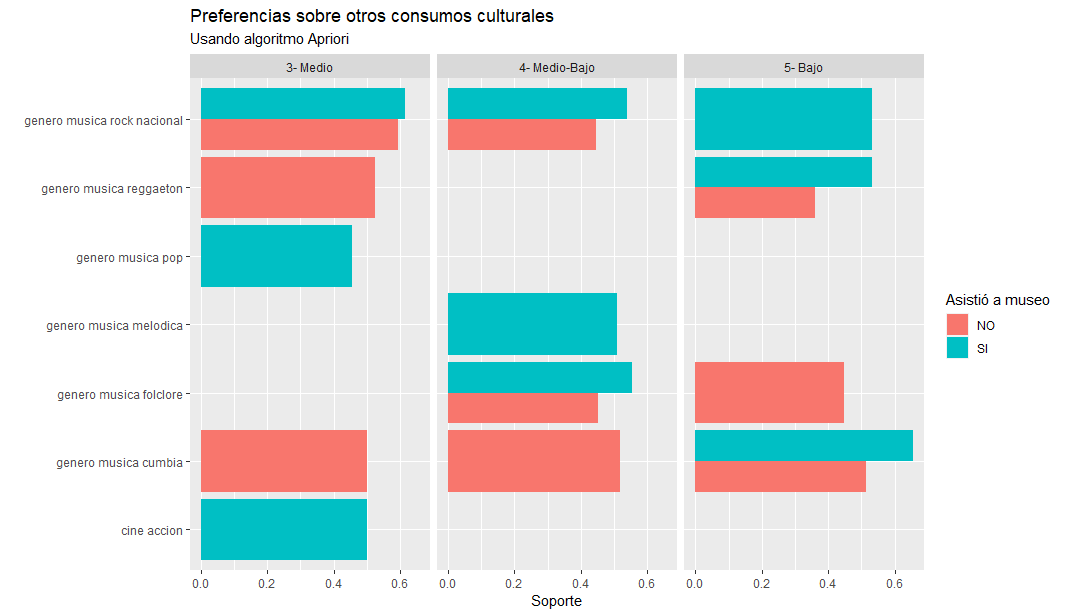
\includegraphics[width=\textwidth]{itemsets.png}
      \label{fig:itemsets}
      \caption{Relación entre otros consumos culturales}
      \end{figure}
    \end{frame}

    \begin{frame}
      \frametitle{Análisis Específico}
      \begin{figure}
        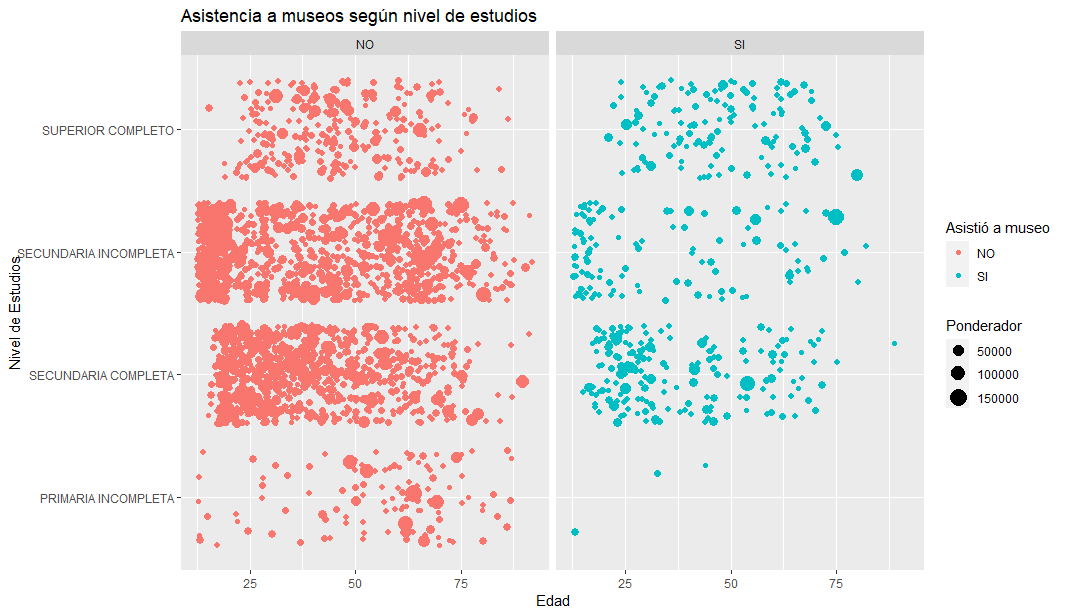
\includegraphics[width=0.95\textwidth]{nivel_estudios.png}
        \label{fig:nivel_estudios}
        \caption{Visitas a museos y escolaridad}
        \end{figure}
      \end{frame}
    
      \begin{frame}
        \frametitle{Análisis Específico}
    
      
        \begin{figure}
          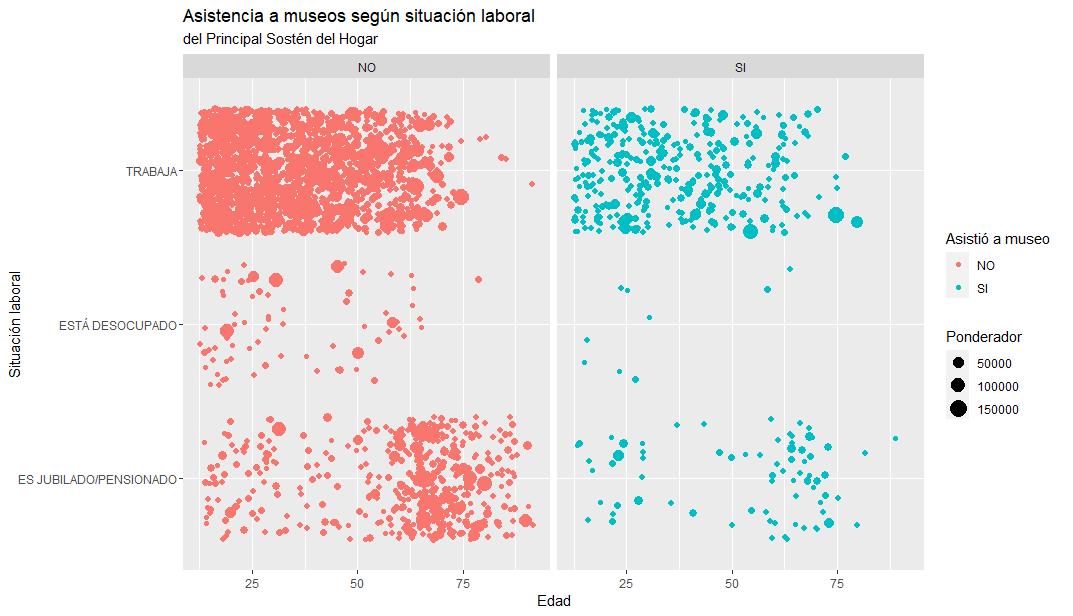
\includegraphics[width=\textwidth]{situacion_psh.png}
          \label{fig:situacion_psh}
          \caption{Visitas a museos y empleo}
          \end{figure}
        \end{frame}

% Cantidad de museos y entradas
\begin{frame}
\frametitle{Modelado}

\begin{figure}
\centering
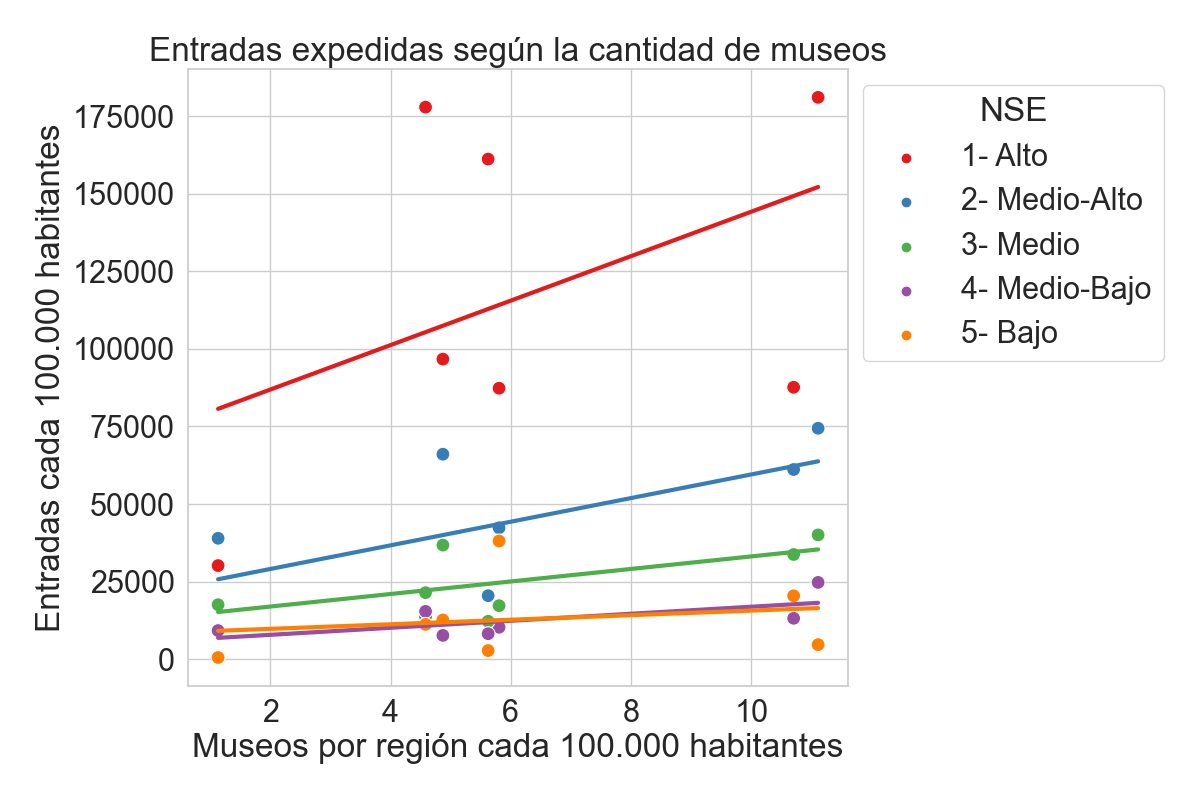
\includegraphics[width=0.9\textwidth]{modelo_entrada_museo}
\label{fig:modelo_entrada_museo}
\caption{Modelo. Multiple R-squared: 0.7544, Adjusted R-squared: 0.6659 }
\end{figure}

\end{frame}

\begin{frame}
  \frametitle{Conclusiones}
  \begin{itemize}
    \item El contexto socio-económico es muy influyente en la concurrencia a museos.
    \item La encuesta podría indagar en las razones de no concurrencia a museos.
    \item Hay una oportunidad de incrementar la concurrencia con las visitas a museos.
    \item Los consumos culturales tienden a ser más digitales. Los museos pueden tomar la iniciativa.
  \end{itemize}
% - Contexto muy influyente en las NSE más bajas para consumos culturales "costosos" (en dinero y tiempo) [habría que tener gàfico anterior de situaciones laborales vs concurrencia]\\
% - Encuesta podría indagar por razones específicas de no-concurrencia a museos\\
% - Oportunidad de incrementar concurrencia concretamente en visitas de las escuelas [gráfico anterior de no-asistencia respecto de edad y nivel de estudios]\\
% - Tendencia no se revertiría por cantidad de museos, la gente de NSE más bajas no se acerca a los museos aún si hay mayor cantidad. Los museos pueden acercarse a la gente (nuevos tipos de museos: interactivos?) [gráfico de uso de redes sociales]
\end{frame}

{
\usebackgroundtemplate{
  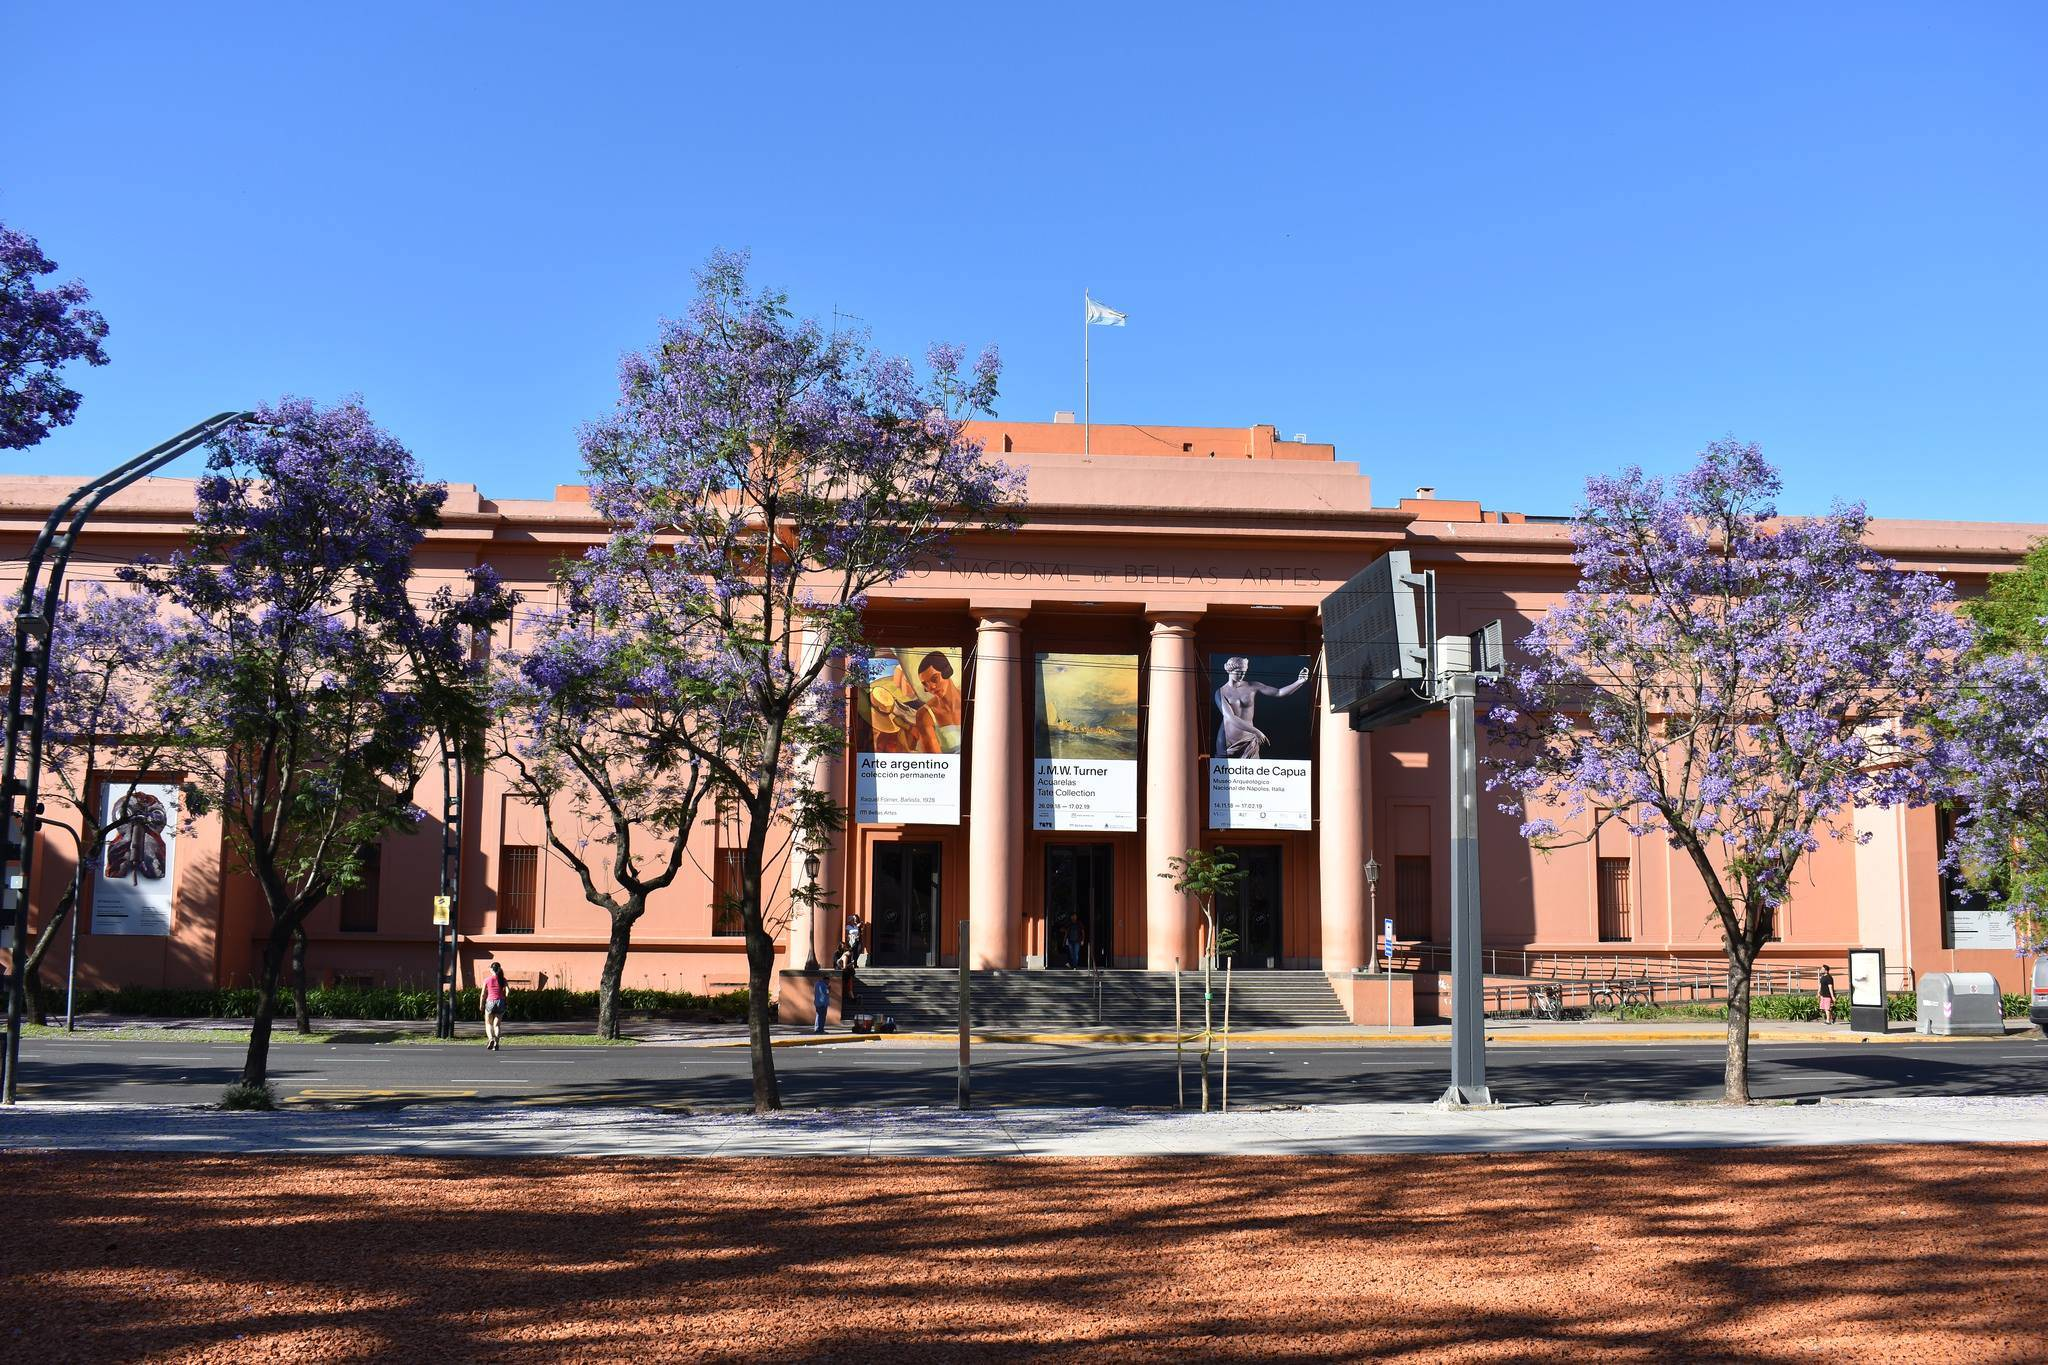
\includegraphics[width=1.2\paperwidth]{mnba-frente.jpg}}%
\begin{frame}
  \frametitle{¡Gracias!}
\vspace{15em}
  \begin{alertblock}{Vayan a los museos}
  ¡Gracias por su atención!\\
  ¿Alguna pregunta?
  \end{alertblock}
  \end{frame}
\end{frame}
}



\begin{frame}
  \frametitle{Fuentes}
  \begin{itemize}
    \item \href{https://datos.cultura.gob.ar/dataset/encuesta-nacional-de-consumos-culturales-2017}{ENCC 2017, Ministerio de Cultura}\\
    \item \href{https://datos.gob.ar/dataset/jgm-servicio-normalizacion-datos-geograficos/archivo/jgm_8.26}{Servicio de Normalización de Datos Geográficos, IGN}
    \item \href{https://datos.gob.ar/dataset/cultura-mapa-cultural-espacios-culturales}{Mapa de Espacios Culturales, Ministerio de Cultura}
  \end{itemize}
  
\end{frame}


\begin{frame}
  \frametitle{Valores del modelo}
\begin{block}{Modelo lineal}
  $entradas\_por\_hab =  museos\_por\_hab \times NSEdenom$
\end{block} 

Residuals:
\resizebox{4cm}{!}{%
  \begin{tabular}{lllll}
  Min    & 1Q    & Media & 3Q   & Max   \\
  -61626 & -9130 & -812  & 5634 & 72512 \\
         &       &       &      &      
  \end{tabular}
}

Coefficients:
\resizebox{\textwidth}{!}{%
  \begin{tabular}{lllll}
                                         &          &            &         &                       \\
                                         & Estimate & Std. Error & t value & Pr(\textgreater{}|t|) \\
  (Intercept)                            & 72552    & 22640      & 3.205   & 0.00367 **            \\
  museos\_por\_hab                       & 7165     & 3204       & 2.236   & 0.03453 *             \\
  NSEdenom2- Medio-Alto                  & -51114   & 32017      & -1.596  & 0.12295               \\
  NSEdenom3- Medio                       & -59638   & 32017      & -1.863  & 0.07430 .             \\
  NSEdenom4- Medio-Bajo                  & -66971   & 32017      & -2.092  & 0.04678 *             \\
  NSEdenom5- Bajo                        & -64255   & 32017      & -2.007  & 0.05569 .             \\
  museos\_por\_hab:NSEdenom2- Medio-Alto & -3356    & 4532       & -0.740  & 0.46590               \\
  museos\_por\_hab:NSEdenom3- Medio      & -5145    & 4532       & -1.135  & 0.26705               \\
  museos\_por\_hab:NSEdenom4- Medio-Bajo & -6033    & 4532       & -1.331  & 0.19510               \\
  museos\_por\_hab:NSEdenom5- Bajo       & -6429    & 4532       & -1.419  & 0.16836              
  \end{tabular}
}


Residual standard error: 27740 on 25 degrees of freedom
Multiple R-squared:  0.7544,	Adjusted R-squared:  0.6659 
F-statistic: 8.531 on 9 and 25 DF,  p-value: 0.00001021
  
\end{frame}


\end{document}
